\documentclass{article}
\usepackage[utf8]{inputenc}

\title{Chem-131C-Lec14}

\author{swflynn }
\date{May 2017}

\usepackage{natbib}
\usepackage{graphicx}
\usepackage{braket}
\usepackage{amsmath}
\usepackage[margin=0.7in]{geometry}
\usepackage{subfigure}
\usepackage{url}
\usepackage{float}

\begin{document}

\maketitle

\section*{Lecture 14; 5/3/17}
The exam is next Friday....You should be studying!
This is the final lecture that will be covered on the exam (the Carnot Cycle is the last topic). 
Note; I have taken the material from 5/5/17 that will be on the exam and incorporated it here, so this is the last lecture you will need for exam preparation.

\subsection*{Adiabatic Processes}
We were able to determine a formula for calculating the entropy of a system, if it is an ideal gas and we know the initial and final V,T (see lecture 8).
\begin{equation}
    S = nR\ln\left[ \left(\frac{T}{T_0} \right)^{3/2} \left(\frac{V}{V_0} \right) \right ] + n\bar{S_0}
\end{equation}

For the adiabatic expansion we can write 
\begin{equation}
    T^{\#}V = constant
\end{equation}

Where the \# depends on the type of idea gas you are working with.

Consider an adiabatic reversible compression of a monoatomic gas. 
However the definition of entropy for this course is
\begin{equation}
    S \equiv \frac{q_{rev}}{T}
\end{equation}
For the adiabatic compression there is no heat transferred therefore the entropy change of the system is 0. 
If we do our expansion from V $\rightarrow$ 2V then
\begin{equation}
    T_f = T2^{\frac{2}{3}}
\end{equation}
The internal energy for an ideal gas is only a function of temperature. 
\begin{equation}
\begin{split}
    U(T) &= \frac{3}{2}nRT \\
    \Delta U &= \frac{3}{2}nRT(2^{\frac{2}{3}}-1)
    \end{split}
\end{equation}

Consider the same question, however, we do the compression irreversibly. 
The final temperature would need to be higher than the reversible case. 
The irreversible case uses excess work to complete the compression in finite time, therefore increasing the energy of the particles in the gas, and consequently increasing the temperature of the gas. 

\subsection*{Carnot Cycle; Last Topic for Midterm}
The Carnot cycle is a very famous engine used to illustrate the concept of efficiency in engineering. 
We know from the first law that U = Q + W, and we know that our state functions must be 0 over a closed cycle $\oint ds = 0$, $\oint dU = 0$, $\oint \delta q \neq 0$, $\oint \delta w \neq 0$.
So we are going to need to prove that that internal energy and entropy are 0 over 1 cycle of the engine, and determine the heat/work associated with each of the four steps in 1 cycle. 

\begin{figure}[H]
    \centering
    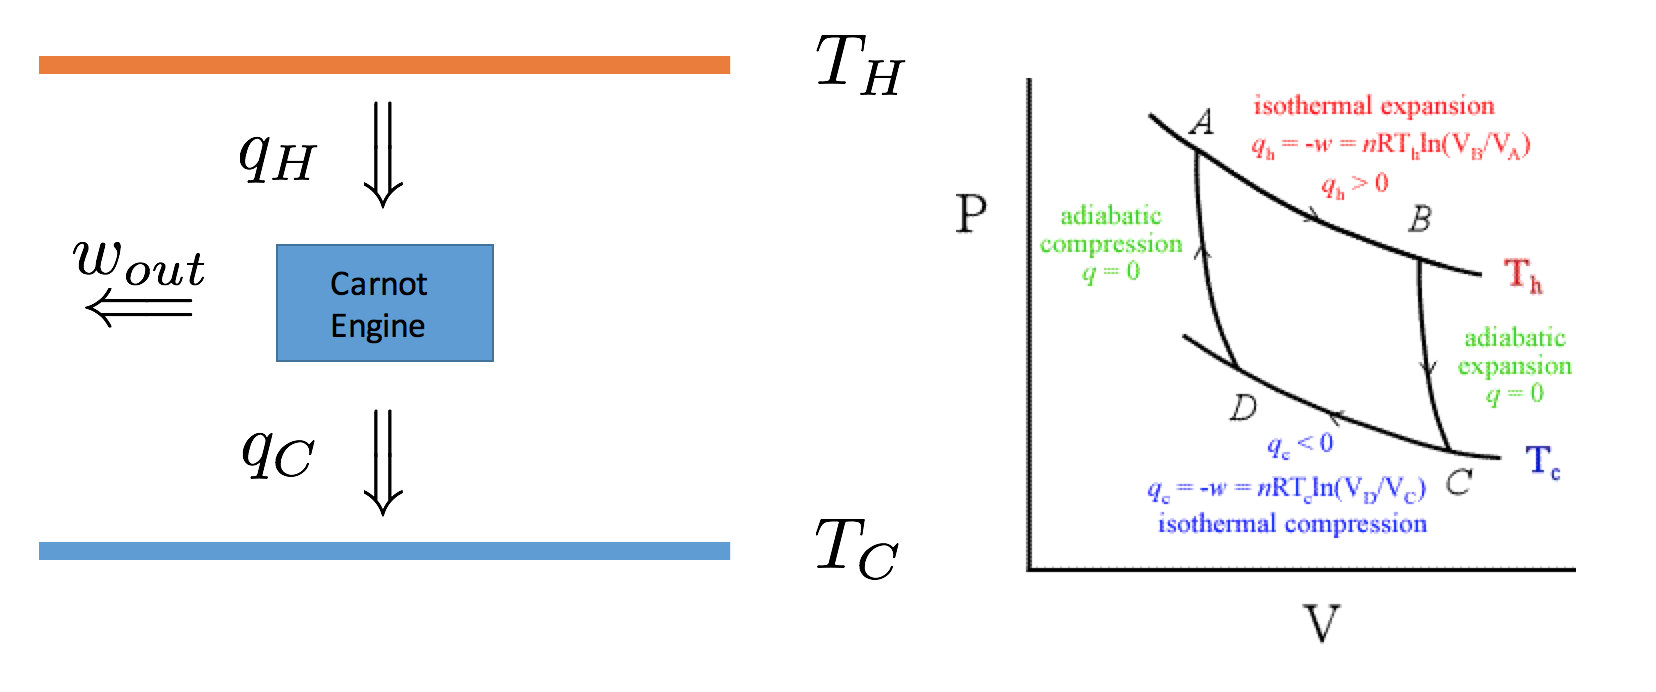
\includegraphics[width=17cm]{carnot.png}
    \caption{Carnot Cycle. The Carnot Cycle we will consider contains 2 reversible isothermal steps and 2 isothermal adiabatic steps (for an ideal gas).}
    \label{fig:carnot}
\end{figure}

\begin{enumerate}
    \item A $\rightarrow$ B is an isothermal expansion at T$_H$. 
    \item B $\rightarrow$ C is an adiabatic expansion, q = 0. 
    \item C $\rightarrow$ D is an isothermal compression at T$_C$. 
    \item D $\rightarrow$ A is an adiabatic compression, q = 0.     
\end{enumerate}

\subsubsection*{A $\rightarrow$ B; Reversible Isothermal Expansion at T$_H$}
Because this expansion is done isothermally with an ideal gas, the internal energy must be 0, so the first law states q = -W. 
We next note that the process is done reversibly so we can substitute in our ideal gas law.
This step is occurring at the higher temperature, therefore this heat must be the heat at the higher temperature (q$_H$) in our generic engine diagram. 
\begin{equation}
\begin{split}
W_{AB} &= -\int_A^B P_{ext}dV = -\int_A^B \frac{nRT_H}{V}dV = -nRT\ln\left(\frac{V_B}{V_A}\right) \\
q_{AB} &= q_H = nRT_H\ln\left(\frac{V_B}{V_A}\right) \\
\Delta S_{AB} &= \frac{q_{r}}{T} = \frac{q_H}{T_H} = nR\ln\left(\frac{V_B}{V_A}\right)
\end{split}
\end{equation}
The sign of q should be positive during this step, the temperature at the beginning is large, the heat enters our engine which we will use to get some useful work out of the system. 

\subsubsection*{B $\rightarrow$ C; Reversible Adiabatic Expansion q = 0}
We are now doing a further expansion adiabatically, q$_{BC}$ = 0 by definition, therefore the temperature must change. 
This means the entropy change for this process is also 0, $\Delta$S$_{BC}$ = 0.

\textbf{Entropy Comment}

As a side comment do not be confused by entropy, we are reversibly expanding the gas, so although the volume is getting larger (which implies an increase in entropy) we are dong the expansion reversibly so the second law definition applies. 
If this were not a reversible expansion (free expansion into a vacuum is not reversible) than the entropy would increase. 
Another way to think about this, the entropy of the universe for a reversible process is 0. 
There is no heat getting into the environment, therefore the entropy of the environment does not change. 
If this is true than the entropy of our process better not change or we would increase the entropy of the universe (and it would no longer be a reversible process). 

Because we are expanding we expect the temperature to decrease if no heat enters the system (the molecules have farther to travel so the average energy decreases). 
Because the process is done adiabatically we know that we can write the first law as U = W.
For an ideal gas (assume monoatomic) the equipartition theorem tells us that
\begin{equation}
\begin{split}
    U(T) &= \frac{3}{2}kT = \frac{3}{2}nRT \\
    \Delta U_{BC}(T) &= \frac{3}{2}nR\Delta T = \frac{3}{2}nR(T_C-T_H)  \\
    W_{BC} &= \frac{3}{2}nR(T_C-T_H) 
\end{split}
\end{equation}

By construction the cold temperature must be lower than the hot temperature, therefore the internal energy decreases during this step. 

\subsubsection*{C $\rightarrow$ D; Reversible Isothermal Compression at T$_C$}
To complete our cycle we must end up at the same initial state, therefore we need to compress our gas (a state is defined by the P,V, T coordinates in this system). 
We are not simply 'rewinding' however, because the heat and work will be unique, specifically we are working at the lower temperature now. 
So yes we are going to put work back into our system, but doing so at a lower temperature will give us a net profit of useful work from the engine cycle.  

\begin{equation}
\begin{split}
\Delta U_{CD} &= 0 \\
W_{CD} &= -nRT_C\ln\left(\frac{V_D}{V_C}\right) \\
q_{CD} &= q_C = nRT_C\ln\left(\frac{V_D}{V_C}\right) \\
\Delta S_{CD} &= \frac{q_C}{T_C} = nR\ln\left(\frac{V_D}{V_C}\right)
\end{split}
\end{equation}

\subsubsection*{D $\rightarrow$ A; Reversible Adiabatic Compression q = 0}
Again from the same argument in the adiabatic expansion the entropy and heat are both 0, and we calculate the change in internal energy (and therefore work) using the equipartition theorem for an ideal gas. 
\begin{equation}
\begin{split}
    q_{DA} &= 0 \\
    \Delta S_{DA} &= 0\\
    \Delta U_{DA} &= \frac{3}{2} nR(T_H-T_C)\\
    W_{DA} &= \frac{3}{2} nR(T_H-T_C)
    \end{split}
\end{equation}

\subsubsection*{Cycle Analysis}
Internal Energy is a state function meaning any path we take will not effect the final result.
Consider each step in our process as the total path.
\begin{equation}
\begin{split}
\Delta U_{cycle} &= U_{AB} + U_{BC} + U_{CD} + U_{DA} \\
& = 0 + \frac{3}{2}nR(T_C-T_H) + 0 + \frac{3}{2}nR(T_H-T_C) = 0
\end{split}
\end{equation}
And as we expect, the internal energy only depends on the initial and final states for a process, if we complete a cycle the initial and final state are the same and we get a $\Delta$ of 0. 

Now repeating the calculation for entropy we find. 
\begin{equation}
\begin{split}
\Delta S_{cycle} &= S_{AB} + S_{BC} + S_{CD} + S_{DA} \\
& =  nR\ln\left(\frac{V_B}{V_A}\right) + 0 +  nR\ln\left(\frac{V_D}{V_C}\right) + 0 \\
\Delta S_{cycle} &= nR\ln\left(\frac{V_BV_D}{V_AV_C}\right)
\end{split}
\end{equation}

To simplify this last line we note that an adiabatic expansion/compression can be characterized by T$^\#$V = constant. 
So consider a ratio between our two temperatures during the adiabatic processes at both the beginning and end of the expansion/compression.
\begin{equation}
\begin{split}
T(A)V(A) \propto T(D)V(D) &\implies \frac{T^{\frac{3}{2}}_H}{T^{\frac{3}{2}}_C} = \frac{V_D}{V_A}\\
T(B)V(B) \propto T(C)V(C) &\implies \frac{T^{\frac{3}{2}}_H}{T^{\frac{3}{2}}_C} = \frac{V_C}{V_B}\\ 
&\implies\\
\frac{V_D}{V_A} &= \frac{V_C}{V_B} \implies \frac{V_BV_D}{V_AV_C} = 1
\end{split}
\end{equation}
And with this comparison we also shown that the entropy of the entire cycle must be 0 (ln[1] = 0). 

As expected we have shown that our state functions both go to 0, it is now time to consider the path functions. 

\begin{equation}
\begin{split}
    W_{cycle} &= -nRT_H\ln\frac{V_B}{V_A} + \frac{3}{2} nR(T_C-T_H) + -nRT_C\ln\frac{V_D}{V_C} + \frac{3}{2} nR(T_H-T_C) \\
    &= -nRT_H\ln\frac{V_B}{V_A} + -nRT_C\ln\frac{V_A}{V_B} \\
    W_{out}&= -nR\ln\frac{V_B}{V_A}(T_H-T_C)
\end{split}
\end{equation}
We note that the total work is negative, this means our system DID work on the surroundings (we got useful work out of the engine). 
So the larger in magnitude we make this number the more we can get out of our engine. 

Let's now look at our heat, we know q$_H$ enters our system (positive value with our convention), and q$_c$ leaves our system to satisfy the second law (so this will be negative in our convention). 
We are going to use our relationship between the volumes from above to put everything in terms of A and B for the sake of comparison. 
\begin{equation}
\begin{split}
    q_H &= q_{AB} = nRT_H \ln \left(\frac{V_B}{V_A}\right)\\
    q_C &= q_{CD} = nRT_C \ln \left(\frac{V_D}{V_C}\right) = -nRT_C \ln \left(\frac{V_B}{V_A}\right) 
\end{split}
\end{equation}

If we now consider the first law we know that 
\begin{equation}
q_C = q_H + W_{out} \implies q_H = q_C + W_{out}
\end{equation}
And if you plug in our expressions from above and do the algebra this relationship holds true. 

Finally if we consider our second law, we know the entropy change of the cycle is 0, we define the entropy of the environment as simply the heat that enters it divided by the temperature (what heat enters/leaves each reservoir). 
\begin{equation}
\Delta S_{univ} = \Delta S_{cycle} + \Delta S_{H,res} + \Delta S_{C,res} = 0 + \frac{-q_H}{T_H} + \frac{q_C}{T_C} = -nR\ln\frac{V_B}{V_A} + nR\ln\frac{V_B}{V_A} = 0
\end{equation}

And again as expected for all reversible processes we did not change the entropy of the universe over the entire cycle. 

\subsection*{Second Law General Statement}
In general we do not expect the entropy of the universe to stay constant, this is only true in the reversible case. 
\begin{equation}
\Delta S_{univ} = \frac{Q_C}{T_C} - \frac{Q_H}{T_H} \geq 0
\end{equation}

This implies a new definition of the second law, this is how entropy is introduced in most engineering thermodynamic courses.
This formulation enforces the fact that an irreversible process must increase the entropy of the universe. 

\begin{equation}
Q_C \geq \frac{T_C}{T_H}q_H
\end{equation}

Where the equality would be the minimum q$_C$. 
We could also cast this in terms of the work instead. 
\begin{equation}
W_{out}^{max} = q_H - q_C^{min} = q_H\left(1-\frac{T_C}{T_H}\right) = q_H\eta
\end{equation}
Here we have defined the thermodynamic efficiency: $\eta = \left(1-\frac{T_C}{T_H}\right) = \frac{W_{out}^{max}}{q_H}$. 

With this analysis completed we have covered all of the material that will be on exam 1, best of luck!

\end{document}